% --
% feature selection

\section{Experiments on MFCC Feature Selection}\label{sec:exp_fs}
\thesisStateNotReady
Feature selection is a very important step prior to neural network training.
The reduction of input features always means a reduction of computations and is therefore a crucial point to evaulate.
Unfortunately it is not always clear, which feature are contributing to good classification scores and which do not or even worsen them.
In this section only Mel Frequency Cepstral Coefficients (MFCC) and their enhancements, as described in \rsec{signal_mfcc}, are the focus of the experiments.
A feature selection for raw audio samples, used in the Wavenet architecture, would not make much sense, because each sample is an feature itself on the time axis.
Another important aspect in the feature selection experiments is the evaluation of the proposed frame-based normalization \req{signal_mfcc_norm} originally applied to improve the visualization of MFCCs and making Generative Adversarial Neural Networks (GANs) more easy and faster to train.
However frame-based normalization might be critical, because it is a normalization done only on the frame (time) scale and disregards the frequency dimension.

Two experiments are done to shade some light into MFCC feature selection:
\begin{enumerate}
    \item Impact on the amount of cepstral coefficients
    \item Impact on the enhancements of MFCCs
\end{enumerate}
For saving training time and computations, those experiments were done on a smaller subset of the whole speech commands dataset, described in \rsec{exp_dataset_speech_cmd}, using 500 samples of each one of the L12 labels.
The filter bands of the MFCCs are fixed to a total number of 32 bands for all experiments.
The training of one set of selected parameters was done with 5 consecutive iterations to create better statistics of the scores.
The scores obtained from those iterations for each set parameters are presented with a mean value and the standard deviation (square root of the variance).

Note that the experiments in this sections are not meant for comparison to the benchmark networks in \rsec{prev_kws_benchmark}, because not the whole dataset is used.


% --
% cepstral

\subsection{Impact on the Amount of Cepstral Coefficients}
The number of cepstral coefficients is selected to either 12 or 32, where a number 12 coefficients is commonly applied in many papers.
The experiments are done once with and once without frame-based normalization to observe its impact on the classification accuracy, the noise and shift invariance.
The standard set of training hyperparameters was used as listed in \rsec{exp_details_training}.
The obtained accuracies on the test set after a training of 2000 epochs are shown in \rtab{exp_fs_cepstral_l12}.
\begin{table}[ht!]
\begin{center}
\caption{Experiment on the impact of the amount of cepstral coefficient of MFCC features with additional frame based normalization evaluation.}
\begin{tabular}{ M{3cm}  M{2cm}  M{2cm}  M{2.5cm}  M{2.5cm} }
\toprule
\textbf{arch} & \textbf{mfcc} & \textbf{norm} & \textbf{acc test} & \textbf{acc my} \\
\midrule
conv-trad & mfcc32-12 & 0 & $81.73 \pm 1.58$ & $80.80 \pm 5.88$ \\
conv-trad & mfcc32-12 & 1 & $75.97 \pm 1.15$ & $90.40 \pm 4.80$ \\
conv-trad & mfcc32-32 & 0 & $80.90 \pm 0.81$ & $81.60 \pm 7.84$ \\
conv-trad & mfcc32-32 & 1 & $74.93 \pm 1.09$ & $88.80 \pm 5.31$ \\
\midrule
conv-fstride & mfcc32-12 & 0 & $74.03 \pm 0.87$ & $73.60 \pm 8.62$ \\
conv-fstride & mfcc32-12 & 1 & $66.33 \pm 1.29$ & $79.20 \pm 6.40$ \\
conv-fstride & mfcc32-32 & 0 & $72.07 \pm 2.24$ & $72.80 \pm 8.54$ \\
conv-fstride & mfcc32-32 & 1 & $63.63 \pm 1.15$ & $91.20 \pm 1.60$ \\
\midrule
conv-jim & mfcc32-12 & 0 & $78.73 \pm 1.55$ & $76.00 \pm 6.69$ \\
conv-jim & mfcc32-12 & 1 & $71.77 \pm 1.77$ & $73.60 \pm 5.43$ \\
conv-jim & mfcc32-32 & 0 & $76.43 \pm 1.52$ & $83.20 \pm 2.99$ \\
conv-jim & mfcc32-32 & 1 & $65.73 \pm 1.94$ & $67.20 \pm 6.88$ \\
\bottomrule
\label{tab:exp_fs_cepstral_l12}
\end{tabular}
\end{center}
\end{table}
\FloatBarrier
\noindent
Note that no early stopping meachanism was applied and the model parameters from the last epoch were used.
In \rfig{exp_fs_cepstral_acc} the accuracies on the validation set of the best performing training instances for each model are shown, where the accuracies are smoothened by a striding average filter with a length of 10 epochs for better visualization.
\begin{figure}[!ht]
  \centering
  \subfigure[conv-trad]{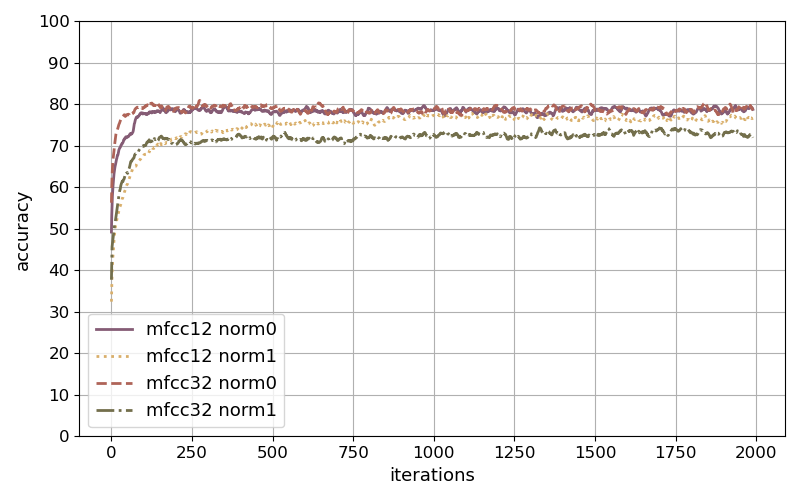
\includegraphics[width=0.45\textwidth]{./5_exp/figs/exp_fs_cepstral_acc_conv-trad}}
  \subfigure[conv-fstride]{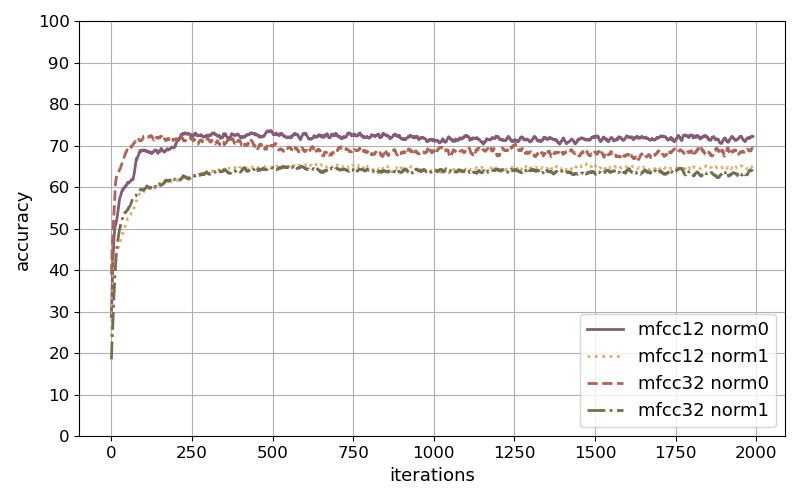
\includegraphics[width=0.45\textwidth]{./5_exp/figs/exp_fs_cepstral_acc_conv-fstride}}
  \subfigure[conv-jim]{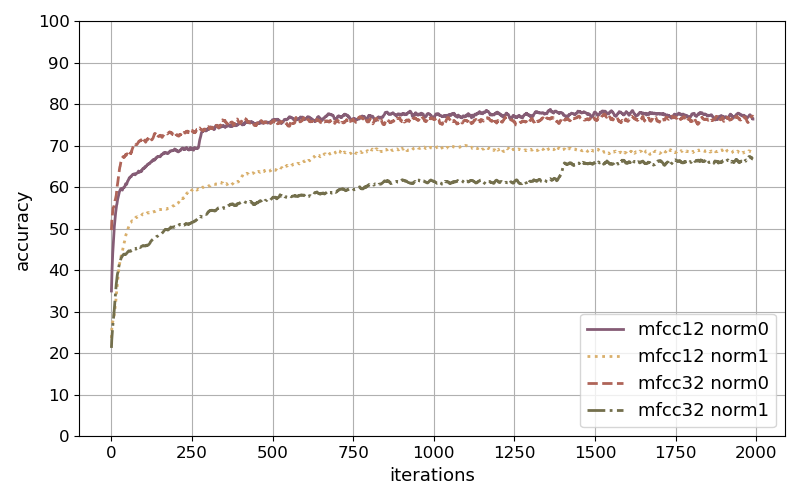
\includegraphics[width=0.45\textwidth]{./5_exp/figs/exp_fs_cepstral_acc_conv-jim}}
  \caption{Accuracies on the validation set of all three CNN models, with different amounts of cepstral coefficients and with and without frame-based normalization.}
  \label{fig:exp_fs_cepstral_acc}
\end{figure}
\FloatBarrier
\noindent

Noise invariance:
\begin{figure}[!ht]
  \centering
  \subfigure[mfcc12, norm0]{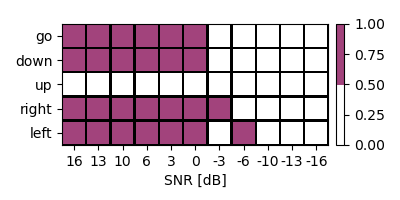
\includegraphics[width=0.35\textwidth]{./5_exp/figs/exp_fs_cepstral_tb_noise_conv-trad_mfcc12_norm0}}
  \subfigure[mfcc12, norm1]{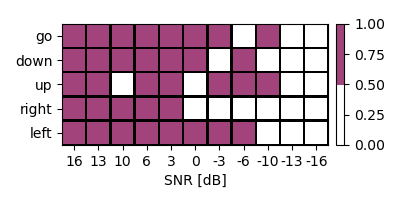
\includegraphics[width=0.35\textwidth]{./5_exp/figs/exp_fs_cepstral_tb_noise_conv-trad_mfcc12_norm1}}
  \subfigure[mfcc32, norm0]{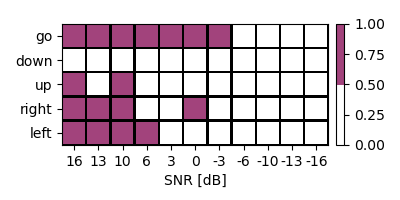
\includegraphics[width=0.35\textwidth]{./5_exp/figs/exp_fs_cepstral_tb_noise_conv-trad_mfcc32_norm0}}
  \subfigure[mfcc32, norm1]{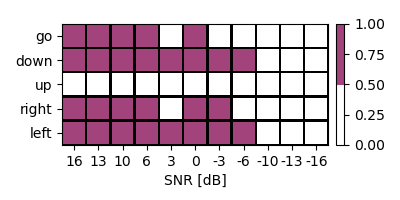
\includegraphics[width=0.35\textwidth]{./5_exp/figs/exp_fs_cepstral_tb_noise_conv-trad_mfcc32_norm1}}
  \caption{Noise invariance of the \texttt{conv-trad} model, with different amounts of cepstral coefficients and with and without frame-based normalization.}
  \label{fig:exp_fs_cepstral_tb_noise_conv-trad}
\end{figure}
\FloatBarrier
\noindent

Shift invariance:
\begin{figure}[!ht]
  \centering
  \subfigure[mfcc12, norm0]{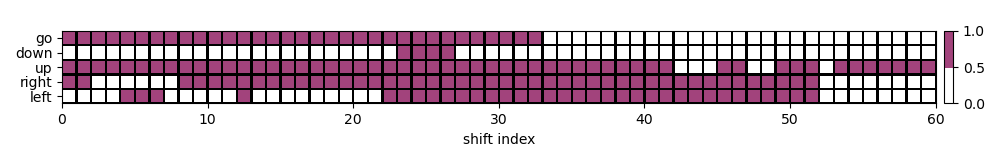
\includegraphics[width=0.45\textwidth]{./5_exp/figs/exp_fs_cepstral_tb_shift_conv-trad_mfcc12_norm0}}
  \subfigure[mfcc12, norm1]{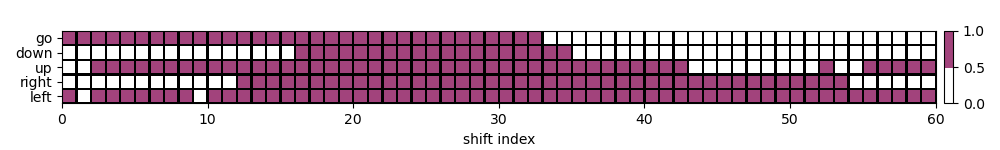
\includegraphics[width=0.45\textwidth]{./5_exp/figs/exp_fs_cepstral_tb_shift_conv-trad_mfcc12_norm1}}
  \subfigure[mfcc32, norm0]{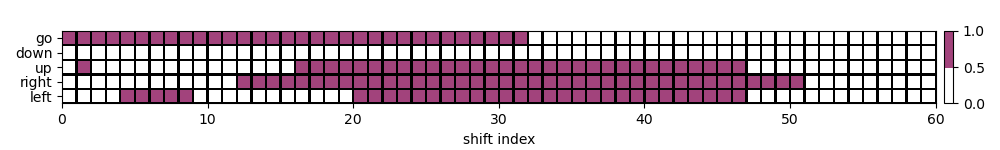
\includegraphics[width=0.45\textwidth]{./5_exp/figs/exp_fs_cepstral_tb_shift_conv-trad_mfcc32_norm0}}
  \subfigure[mfcc32, norm1]{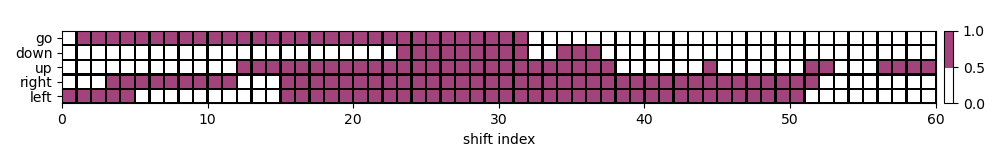
\includegraphics[width=0.45\textwidth]{./5_exp/figs/exp_fs_cepstral_tb_shift_conv-trad_mfcc32_norm1}}
  \caption{Shift invariance of the \texttt{conv-trad} model, with different amounts of cepstral coefficients and with and without frame-based normalization.}
  \label{fig:exp_fs_cepstral_tb_noise_conv-trad}
\end{figure}
\FloatBarrier
\noindent

Noise invariance:
\begin{figure}[!ht]
  \centering
  \subfigure[mfcc12, norm0]{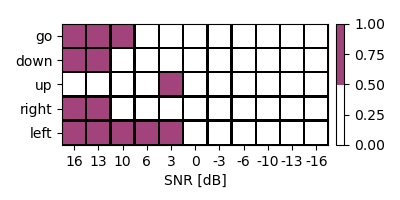
\includegraphics[width=0.35\textwidth]{./5_exp/figs/exp_fs_cepstral_tb_noise_conv-fstride_mfcc12_norm0}}
  \subfigure[mfcc12, norm1]{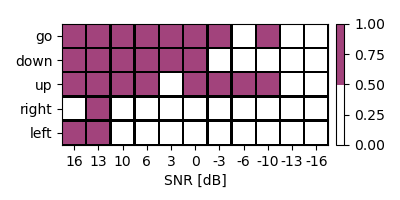
\includegraphics[width=0.35\textwidth]{./5_exp/figs/exp_fs_cepstral_tb_noise_conv-fstride_mfcc12_norm1}}
  \subfigure[mfcc32, norm0]{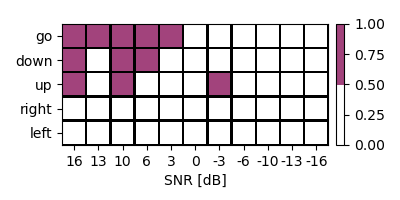
\includegraphics[width=0.35\textwidth]{./5_exp/figs/exp_fs_cepstral_tb_noise_conv-fstride_mfcc32_norm0}}
  \subfigure[mfcc32, norm1]{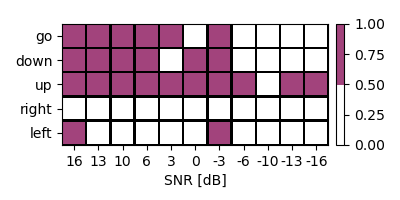
\includegraphics[width=0.35\textwidth]{./5_exp/figs/exp_fs_cepstral_tb_noise_conv-fstride_mfcc32_norm1}}
  \caption{Noise invariance of the \texttt{conv-fstride} model, with different amounts of cepstral coefficients and with and without frame-based normalization.}
  \label{fig:exp_fs_cepstral_tb_noise_conv-fstride}
\end{figure}
\FloatBarrier
\noindent

Shift invariance:
\begin{figure}[!ht]
  \centering
  \subfigure[mfcc12, norm0]{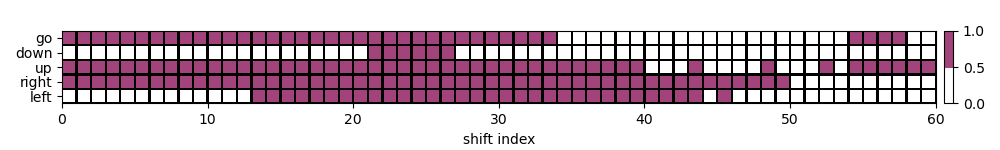
\includegraphics[width=0.45\textwidth]{./5_exp/figs/exp_fs_cepstral_tb_shift_conv-fstride_mfcc12_norm0}}
  \subfigure[mfcc12, norm1]{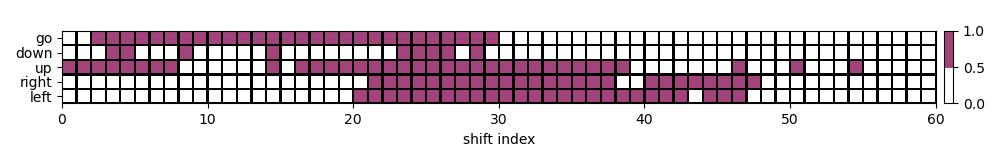
\includegraphics[width=0.45\textwidth]{./5_exp/figs/exp_fs_cepstral_tb_shift_conv-fstride_mfcc12_norm1}}
  \subfigure[mfcc32, norm0]{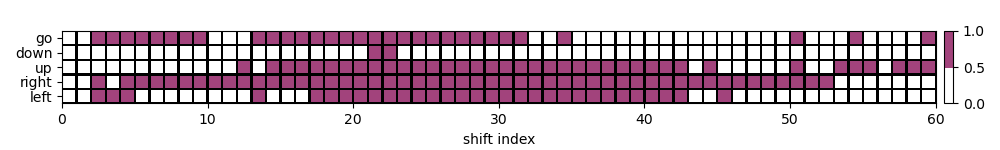
\includegraphics[width=0.45\textwidth]{./5_exp/figs/exp_fs_cepstral_tb_shift_conv-fstride_mfcc32_norm0}}
  \subfigure[mfcc32, norm1]{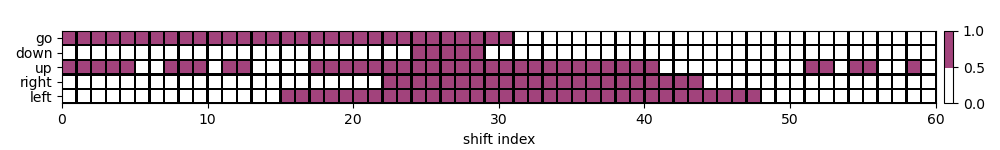
\includegraphics[width=0.45\textwidth]{./5_exp/figs/exp_fs_cepstral_tb_shift_conv-fstride_mfcc32_norm1}}
  \caption{Shift invariance of the \texttt{conv-fstride} model, with different amounts of cepstral coefficients and with and without frame-based normalization.}
  \label{fig:exp_fs_cepstral_tb_noise_conv-fstride}
\end{figure}
\FloatBarrier
\noindent

Noise invariance:
\begin{figure}[!ht]
  \centering
  \subfigure[mfcc12, norm0]{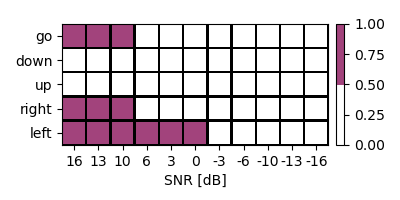
\includegraphics[width=0.35\textwidth]{./5_exp/figs/exp_fs_cepstral_tb_noise_conv-jim_mfcc12_norm0}}
  \subfigure[mfcc12, norm1]{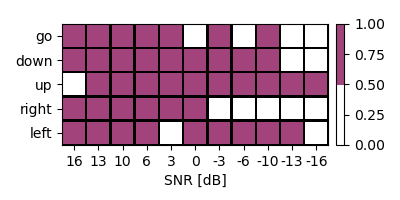
\includegraphics[width=0.35\textwidth]{./5_exp/figs/exp_fs_cepstral_tb_noise_conv-jim_mfcc12_norm1}}
  \subfigure[mfcc32, norm0]{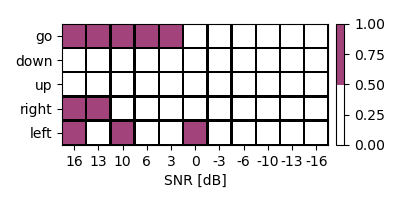
\includegraphics[width=0.35\textwidth]{./5_exp/figs/exp_fs_cepstral_tb_noise_conv-jim_mfcc32_norm0}}
  \subfigure[mfcc32, norm1]{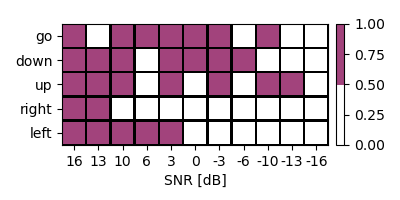
\includegraphics[width=0.35\textwidth]{./5_exp/figs/exp_fs_cepstral_tb_noise_conv-jim_mfcc32_norm1}}
  \caption{Noise invariance of the \texttt{conv-jim} model, with different amounts of cepstral coefficients and with and without frame-based normalization.}
  \label{fig:exp_fs_cepstral_tb_noise_conv-jim}
\end{figure}
\FloatBarrier
\noindent

Shift invariance:
\begin{figure}[!ht]
  \centering
  \subfigure[mfcc12, norm0]{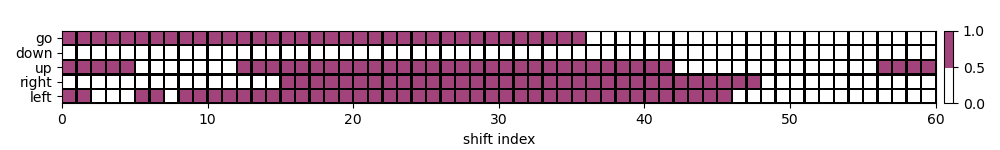
\includegraphics[width=0.45\textwidth]{./5_exp/figs/exp_fs_cepstral_tb_shift_conv-jim_mfcc12_norm0}}
  \subfigure[mfcc12, norm1]{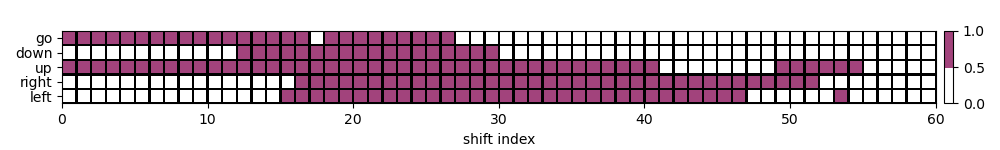
\includegraphics[width=0.45\textwidth]{./5_exp/figs/exp_fs_cepstral_tb_shift_conv-jim_mfcc12_norm1}}
  \subfigure[mfcc32, norm0]{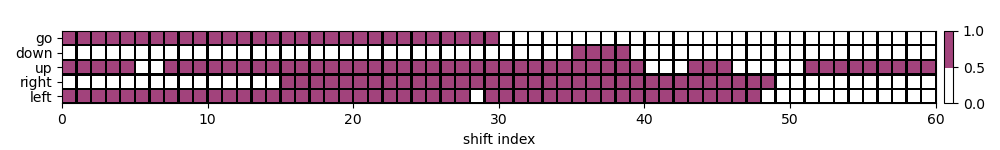
\includegraphics[width=0.45\textwidth]{./5_exp/figs/exp_fs_cepstral_tb_shift_conv-jim_mfcc32_norm0}}
  \subfigure[mfcc32, norm1]{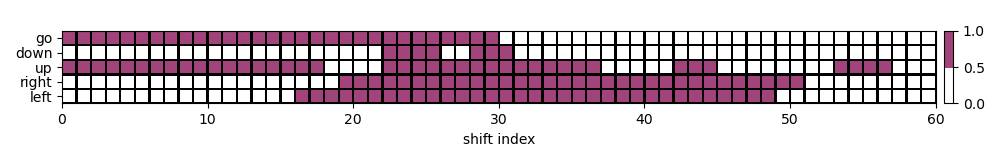
\includegraphics[width=0.45\textwidth]{./5_exp/figs/exp_fs_cepstral_tb_shift_conv-jim_mfcc32_norm1}}
  \caption{Shift invariance of the \texttt{conv-jim} model, with different amounts of cepstral coefficients and with and without frame-based normalization.}
  \label{fig:exp_fs_cepstral_tb_noise_conv-jim}
\end{figure}
\FloatBarrier
\noindent



% --
% enhancements

\subsection{Impact on the enhancements of MFCCs}\label{sec:exp_fs_mfcc}
In this experiment the cepstral coefficients were selected to 12 and enhanced with deltas (d), double deltas (dd) and energy vectors (e) as described in \rsec{signal_mfcc_enhancement}.
The frame-based normalization was applied with results listed in \rtab{exp_fs_mfcc_l12}.
\begin{table}[ht!]
\small
\begin{center}
\caption{Experiment on the impact of feature enhancement of cepstral coefficients (c), deltas (d), double deltas (dd) and energy vectors (e) performed on the \texttt{conv-jim} model with frame-based normalization}
\begin{tabular}{ M{1cm}  M{1cm}  M{1cm}  M{1cm}  M{2.5cm}  M{2.5cm} }
\toprule
\textbf{c} & \textbf{d} & \textbf{dd} & \textbf{e} & \textbf{acc test} & \textbf{acc my} \\
\midrule
0 & 0 & 1 & 0 & $37.40 \pm 2.17$ & $34.40 \pm 11.20$ \\
0 & 0 & 1 & 1 & $46.63 \pm 2.87$ & $36.80 \pm 7.76$ \\
0 & 1 & 0 & 0 & $58.57 \pm 2.06$ & $64.80 \pm 4.66$ \\
0 & 1 & 0 & 1 & $62.00 \pm 1.82$ & $75.20 \pm 11.14$ \\
0 & 1 & 1 & 0 & $59.03 \pm 1.77$ & $56.00 \pm 9.47$ \\
0 & 1 & 1 & 1 & $61.60 \pm 2.28$ & $62.40 \pm 6.97$ \\
1 & 0 & 0 & 0 & $72.00 \pm 1.46$ & $85.60 \pm 1.96$ \\
1 & 0 & 0 & 1 & $72.83 \pm 1.22$ & $80.00 \pm 4.38$ \\
1 & 0 & 1 & 0 & $70.63 \pm 2.13$ & $84.00 \pm 8.76$ \\
1 & 0 & 1 & 1 & $72.36 \pm 2.27$ & $80.00 \pm 4.38$ \\
1 & 1 & 0 & 0 & $72.80 \pm 2.90$ & $88.80 \pm 6.88$ \\
1 & 1 & 0 & 1 & $75.30 \pm 1.38$ & $92.00 \pm 2.53$ \\
1 & 1 & 1 & 0 & $73.43 \pm 2.05$ & $84.80 \pm 5.88$ \\
1 & 1 & 1 & 1 & $73.73 \pm 1.66$ & $83.20 \pm 6.88$ \\
\bottomrule
\label{tab:exp_fs_mfcc_l12}
\end{tabular}
\end{center}
\vspace{-4mm}
\end{table}
\FloatBarrier
\noindent
The best two feature enhancements were used for examining the noise and shift invaiance, those enhancements were the full MFCC-39 features and the (c, d, e) features.

acc:
\begin{figure}[!ht]
  \centering
  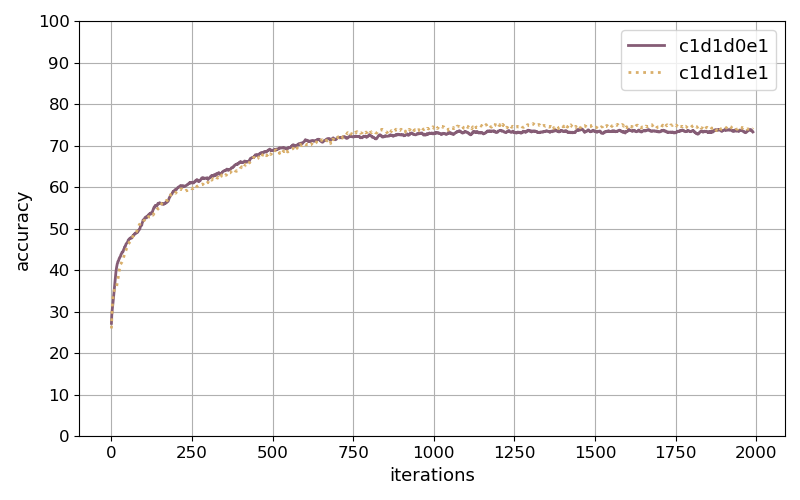
\includegraphics[width=0.45\textwidth]{./5_exp/figs/exp_fs_mfcc_acc_conv-jim}
  \caption{Accuracies of the \texttt{conv-jim} model, with different feature enhancements and frame-based normalization.}
  \label{fig:exp_fs_mfcc_tb_acc_conv-jim}
\end{figure}
\FloatBarrier
\noindent


Noise invariance:
\begin{figure}[!ht]
  \centering
  \subfigure[mfcc-39]{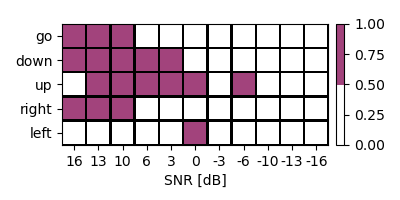
\includegraphics[width=0.35\textwidth]{./5_exp/figs/exp_fs_mfcc_tb_noise_conv-jim_c1d1d1e1}}
  \subfigure[c, d, e]{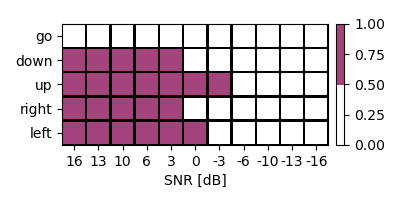
\includegraphics[width=0.35\textwidth]{./5_exp/figs/exp_fs_mfcc_tb_noise_conv-jim_c1d1d0e1}}
  \caption{Noise invariance of the \texttt{conv-jim} model, with different feature enhancements and frame-based normalization.}
  \label{fig:exp_fs_mfcc_tb_noise_conv-jim}
\end{figure}
\FloatBarrier
\noindent

Shift invariance:
\begin{figure}[!ht]
  \centering
  \subfigure[mfcc-39]{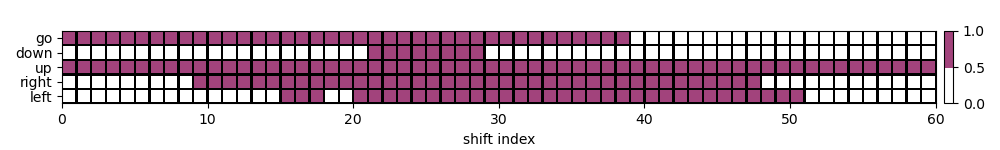
\includegraphics[width=0.45\textwidth]{./5_exp/figs/exp_fs_mfcc_tb_shift_conv-jim_c1d1d1e1}}
  \subfigure[c, d, e]{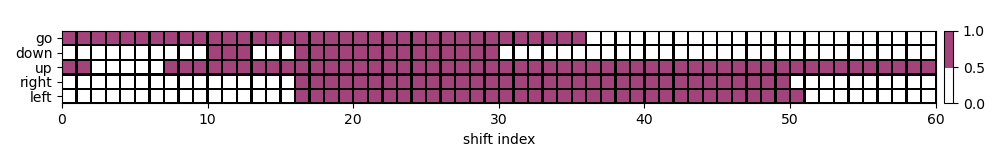
\includegraphics[width=0.45\textwidth]{./5_exp/figs/exp_fs_mfcc_tb_shift_conv-jim_c1d1d0e1}}
  \caption{Shift invariance of the \texttt{conv-jim} model with different feature enhancements and frame-based normalization.}
  \label{fig:exp_fs_mfcc_tb_shift_conv-jim}
\end{figure}
\FloatBarrier
\noindent
